\section{Speculative Execution}
Speculative execution is a technique implemented by the majority of modern CPUs to maximize perfomances. 
As the name suggests, it is based on the execution of operations that might or might not be performed.
In case it's discovered that such instructions shouldn't have had been executed, all results are discarded, and CPU previous state is restored.
For this reason speculatively executed instructions are also referred as transient instructions.
In this section we will give a look at different speculation techniques, to better understand how the different versions of Spectre vulnerability work.

\subsection{Branch Prediction}
READ PIPELINING AND WRITE THIS INTRODUCTION FFS.
\subsubsection{Static Branch Prediction}
Static Branch Prediction is the simplest type of Branch Prediction. Predictor behaviour does not change during the execution of a program. The simplest examples are predictors that either predict that branch are always taken or always not taken. Some ISAs give the possibility, when using branch instructions, to insert a bit that hints wether a branch should be predicted taken or not.
\subsubsection{Dynamic Branch Prediction}
Dynamic Branch Predictors change their prediction based on information gathered at run-time, for an improved misprediction rate. A buffer, called Branch History Table(BHT) or Branch Prediction Buffer(BPB), is used to store predictions.
The table maps a branch instruction address to bits used to store information about predictions' outcome. BHT implementations differ on how the mapping is done(Hash functions, k least significant bits, ...) and the number of bits associated with each address. The simplest way is using a single bit that stores the last outcome of the branch instruction(taken, not taken).
This method doesn't take it count if the last prediction was or wasn't right, plus for every loop it's always wrong at least once. Using 2 bits can fix this problem, how the prediction changes can be summarized by the following state diagram.

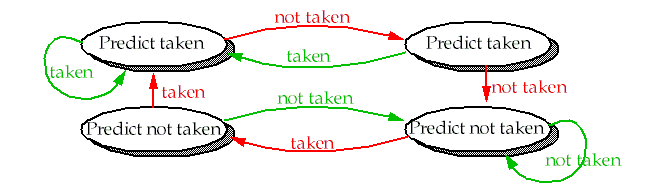
\includegraphics[scale=0.35]{img/2bitBHT.png}

Dynamic Branch Predictor evolved and became more complex, and the concept of 2-level prediction arised. It is based on 2 concepts: Global Branch Correlation, or how a branch outcome is influenced by other branches, and Local Branch Correlation, that is how a branch is influenced by past predictions. This type of prediction uses what's called Patther History Table, or PHT, which associates the pattern(other branches + past outcomes) with the 2-bit schema seen before. This notably enhances the number of correct prediction.
Modern Branch Predictors' PHT use machine learning, state-of-the-art predictors use what's called perceptron predictor. This improves misprediction rate but increases latency. For the sake of this paper we will not dive into this argument.

\subsection{Branch Target Prediction}
Another type of speculation implemented in modern CPUs is Branch Target Prediction.
Every time a jump instruction is encountered fetch cycles are lost to fetch and decode the instruction.
To fasten up this process, in order to fetch the target instruction as soon as possible, modern CPUs implement what's called a Branch Target Predictor.
Branch Target Predictor uses a buffer called Branche Target Buffer(BTB), which structure is analog to a cache: it associates instruction PCs to branch target PCs. Every time a new jump is fetched and decoded, its PC and target address are stored in the BTB.
For every entry in the table 2 predictions bits are added, just like branch prediction 2-bit schema, to improve target prediction.
This means that new entry have 2 prediction bits set as 'Predict Taken'.
Every time an instruction is fetched, the BTB is looked up to check if it contains the instruction PC, if so, then the associated target address is sent out.
If it target turns out to be correct then we've saved - TODO -
If not the entry is deleted from the BTB, and 2 cycles are lost.
If the instruction PC is not in the BTB and after being decoded turns out it's a jump instruction then its PC and target address are saved in the table.
This means that when the same jump instruction is encountered it is recognized as a jump instruction even before fetching it.
Workflow can be seen in Figure underneath:

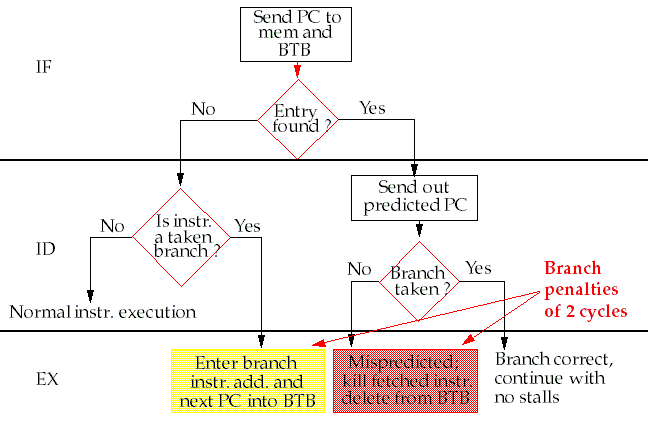
\includegraphics[scale=0.35]{img/BTB.png}

\subsection{Return Address Prediction}
Indirect jumps are jump instructions where the target address is not directly passed, a register or a memory address containing the target is given instead.
This means that once the CU decodes the indirect jump instruction, clock cycles are spent to fetch the address from the register, cache or, worst-case scenario, a cache-miss happens and the target is fetched from main memory.
The majority of this calls are from procedure returns. Even though a Branch Target Predictor could be used in this situation, its accuracy can be low in this situations. A buffer called Return Stack Buffer is used instead. It acts as a stack, so it pushes the latest return address on the stack and pops it off when a return is called.

\subsection{Speculative Store Buffer Bypass}
In order to improve performances, write operations(also called stores) are saved in a high speed buffer called Store Buffer. This allows the CPU to not wait for the buffer to be written back in slower memory.
This implies that every time a read operaton on main memory is done, the CPU must check if a previously store operation on the same address was done and not written back. 
Modern CPUs bypass this check and assume that such stores are already written back, thus proceed to speculatively execute later instructions, and concurrently check the Store Buffer.
If conflicts are found, results of transient instructions are thrown away, otherwise a significant speedup is achieved.
